\SourcePage{236}{239}
\section{Transition probability in the semiclassical case}

Passage through a potential barrier exemplifies a process that cannot occur at
all in classical mechanics. In the semiclassical case, the probability of such
processes is exponentially small. The corresponding exponent can be found as
follows.

Consider a transition of some system from one state to another. We solve the
appropriate classical equations of motion and determine the transition
``trajectory.'' Since the process is impossible in classical mechanics, this
trajectory is complex. In general, the ``transition point'' $q_0$, at which the
system formally passes from one state to the other, is complex as well; its
position is fixed by the classical conservation laws. We next calculate the
action $S_1(q_1,q_0)+S_2(q_0,q_2)$: in the first state the system moves from an
arbitrary initial position $q_1$ to the ``transition point'' $q_0$, and in the
second state it moves from $q_0$ to the final position $q_2$. The probability
of the process is then
\begin{equation}
 w\sim\exp\left\{-\frac2\hbar\operatorname{Im}
 [S_1(q_1,q_0)+S_2(q_0,q_2)]\right\}.
 \tag{52.1}
\end{equation}

If several positions are possible for the ``transition point,'' the one for
which the exponent in (52.1) has the smallest absolute value must be selected
(this value must, of course, still be sufficiently large for (52.1) to be
applicable at all)\footnote{If the potential energy of the system itself has
singular points, these points too must be included among the competing values
of $q_0$.}.

Formula (52.1) agrees with the rule obtained in the preceding section for
calculating semiclassical matrix elements. It should be stressed, however,
that it would be wrong to calculate the pre-exponential factor in the
probability of a transition of this kind by squaring the corresponding matrix
element.

The method of \emph{complex classical trajectories} based on (52.1) is quite
general and applies to transitions in systems having any number of degrees of
freedom (L.~D. Landau,

\SourcePage{237}{240}
1932). When the transition point is real but lies in a classically forbidden
region, formula (52.1), in the simplest case of one-dimensional motion,
coincides with expression (50.5) for the probability of passage through a
potential barrier.

\textbf{Above-barrier reflection.} Let us apply (52.1) to the one-dimensional
problem of above-barrier reflection, in which the energy of the particle
exceeds the height of the barrier. Here $q_0$ is to be understood as the
complex coordinate $x_0$ of the ``stopping point'' where the particle reverses
its direction of motion; thus, $x_0$ is a complex root of $U(x)=E$. We shall
show that in this case the reflection coefficient can also be calculated more
accurately, including its pre-exponential factor.

Once again (as in \S~50), we have to relate the wave functions far on the
right-hand side of the barrier (the transmitted wave) to those far on its
left-hand side (the incident and reflected waves).

We may do this without difficulty by proceeding as in \SS~47 and 50 and
regarding $\psi$ as a function of the complex variable $x$.


Write the transmitted wave as
\[
 \psi_+=\frac1{\sqrt p}\exp\left(\frac i\hbar\int_{x_1}^x p\,dx\right)
\]
(where $x_1$ is any point on the real axis), and follow its change on going
through the upper half-plane along a path $C$ which passes around the turning
point $x_0$ at a sufficient distance (Fig.~19). The final portion of this path
must lie entirely in a region sufficiently far to the left that, along it, the
error in the approximate semiclassical wave function of the incident wave is
smaller than the small quantity $\psi_-$ being sought. Going around $x_0$
changes the sign of the root $\sqrt{E-U(x)}$. Consequently, upon returning to
the real axis, $\psi_+$ becomes a wave $\psi_-$ traveling to the left, that is,
the reflected wave\footnote{A path passing below $x_0$ (for example, simply
along the real axis itself) instead transforms $\psi_+$ into the incident
wave.}. Since the amplitudes of the incident and transmitted waves may be
taken to coincide, the required reflection coefficient $R$ is simply

\begin{figure}[ht]
\centering
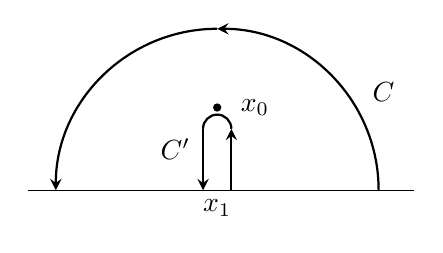
\begin{tikzpicture}[x=1cm,y=1cm,>=stealth]
 \draw (-2.4,0)--(2.5,0);
 \fill (0,1.05) circle (1.5pt) node[right=5pt] {$x_0$};
 \node[below] at (0,0) {$x_1$};
 \draw[thick,->] (2.05,0) arc[start angle=0,end angle=90,radius=2.05];
 \draw[thick,->] (0,2.05) arc[start angle=90,end angle=180,radius=2.05];
 \node[right] at (1.85,1.25) {$C$};
 \draw[thick,->] (0.18,0)--(0.18,.78);
 \draw[thick] (0.18,.78) arc[start angle=0,end angle=180,radius=.18];
 \draw[thick,->] (-.18,.78)--(-.18,0);
 \node[left] at (-.22,.52) {$C'$};
\end{tikzpicture}
\par\smallskip Fig. 19
\end{figure}

\SourcePage{238}{241}
the ratio of the squared moduli of $\psi_-$ and $\psi_+$:
\begin{equation}
 R=\left|\frac{\psi_-}{\psi_+}\right|^2
 =\exp\left(-\frac2\hbar\operatorname{Im}\int_Cp\,dx\right).
 \tag{52.2}
\end{equation}

Once this formula has been obtained, the integration path in the exponent may
be deformed in any manner. If it is changed into the path $C'$ shown in
Fig.~19, the integral reduces to twice the integral along the path from $x_1$
to $x_0$, giving
\begin{equation}
 R=e^{-4\sigma(x_1,x_0)/\hbar},\qquad
 \sigma(x_1,x_0)=\operatorname{Im}\int_{x_1}^{x_0}p(x)\,dx;
 \tag{52.3}
\end{equation}
since $p(x)$ is real everywhere on the real axis, the choice of $x_1$ is
immaterial\footnote{In some cases, not only the amplitude relation but also
the phase relation between the incident and reflected waves is of interest.
These relations are characterized by the reflection amplitude, expressed in
terms of the coefficients $\alpha$ and $\beta$ introduced in \S~25. The
reasoning given above readily shows, in particular, that the reflection
amplitude for a wave incident from the left is
\[
 \left(-\frac{\beta^*}{\alpha^*}\right)
 =-i\exp\left[\frac{2i}{\hbar}\left(
 \int_{x_1}^{x_0}p\,dx+p_1x_1\right)\right],\qquad x_1\to-\infty.
\]
(The factor $(-i)$ is associated with the change in phase of the
pre-exponential factor on going around the branch point; compare \S~47.)}.
Notice that the pre-exponential factor in (52.3) is equal to unity
(V.~L. Pokrovskii, S.~K. Savvinykh, F.~R. Ulinich, 1958)\footnote{The
derivation of this result presented here is due to L.~D. Landau (1961).}.

As stated above, among all possible values of $x_0$ one must choose the value
for which the exponent in (52.3) has the smallest absolute magnitude, while
that magnitude must still be sufficiently large compared with unity. (Only
points $x_0$ for which $\sigma>0$, that is, points in the upper half-plane,
are of course to be considered.) It is also assumed that if the potential
energy $U(x)$ itself has singular points in the upper half-plane, the values of
the integral $\sigma(x_1,x_0)$ for these points are large\footnote{The contour
$C$ in Fig.~19 must be taken below the singular points of $U(x)$.}. Otherwise,
such a point determines the exponent, but the pre-exponential factor will no
longer be the one in (52.3). This last condition is inevitably violated as the
energy $E$ increases if $U(x)$ becomes infinite somewhere

\SourcePage{239}{242}
in the upper half-plane. A stage is reached at which the point $x_0$ where
$U=E$ is so close to the point $x_\infty$ where $U=\infty$ that the two make
comparable contributions to the reflection coefficient (the integral
$\sigma(x_\infty,x_0)\sim1$), and formula (52.3) ceases to apply.
In the limiting regime where $E$ is so large that the indicated integral is
small relative to unity, perturbation theory becomes applicable (see Problem
2)\footnote{The intermediate regime was considered by V.~L. Pokrovskii and
I.~M. Khalatnikov (Zh. Eksp. Teor. Fiz. 1961. Vol.~40. P.~1713).}.

